\documentclass[11pt]{report}
\usepackage[margin=1in]{geometry}
\usepackage[T1]{fontenc}
\usepackage[utf8]{inputenc}
\usepackage{lmodern}
\usepackage{microtype}
\usepackage{amsmath,amssymb,amsfonts,mathtools,bm}
\usepackage{booktabs,longtable,array,multirow}
\usepackage{graphicx}
\usepackage{xcolor}
\usepackage{hyperref}
\usepackage{enumitem}
\usepackage{listings}
\usepackage{algorithm}
\usepackage{algpseudocode}
\usepackage{tikz}
\usetikzlibrary{arrows.meta,positioning,shapes.geometric,shapes.multipart,fit,calc}
\usepackage{float}
\hypersetup{colorlinks=true,linkcolor=blue!60!black,urlcolor=blue!60!black,citecolor=blue!60!black}

\lstset{
  basicstyle=\ttfamily\small,
  backgroundcolor=\color{gray!8},
  frame=single,
  breaklines=true,
  columns=fullflexible
}

\newcommand{\code}[1]{\texttt{#1}}
\newcommand{\km}{\ensuremath{\,\mathrm{km}}}
\newcommand{\dd}{\ensuremath{\,\mathrm{d}}}
\newcommand{\celsius}{\ensuremath{^{\circ}\mathrm{C}}}
\newcommand{\R}{\ensuremath{R_\oplus}}
\newcommand{\Tref}{\ensuremath{T_{26}}}
\newcommand{\OHC}{\ensuremath{\mathrm{OHC}}}
\newcommand{\TCHP}{\ensuremath{\mathrm{TCHP}}}
\newcommand{\Dtwentysix}{\ensuremath{D_{26}}}
\newcolumntype{P}[1]{>{\raggedright\arraybackslash}p{#1}}

\title{HHP Interpolation and Machine-Learning Correction\\Technical Schematic Report}
\author{Prepared from the current codebase in \code{/home/suramya/HHP-Prediction/OHC}}
\date{2026-06-04}

\begin{document}
\maketitle
\tableofcontents

\chapter*{Executive Summary}
\addcontentsline{toc}{chapter}{Executive Summary}
This report documents the current Ocean Heat Content / Tropical Cyclone Heat Potential (OHC/TCHP) workflow used in the HHP project. It explains the TEOS-10 physics calculations, the exact-location Argo--RTOFS collocation design, the interpolation methods and masking rules used for seasonal maps, and the residual-learning machine-learning pipeline that corrects RTOFS toward Argo.

The key scientific point is that raw Argo observations are globally distributed, but valid \Dtwentysix{} and \TCHP{} values only exist where the upper ocean crosses the \(26\celsius{}\) isotherm. The key computational point is that the current strongest correction model is a year-holdout XGBoost residual model trained on 2024 collocated rows and evaluated on 2025 collocated rows.

\chapter{Code Inventory and Project Structure}
\section{Files of Record}
\small
\setlength{\LTleft}{0pt}
\setlength{\LTright}{0pt}
\begin{longtable}{P{0.34\textwidth} P{0.60\textwidth}}
\toprule
\textbf{File} & \textbf{Role in workflow} \\
\midrule
\endhead
\path{OHC/teos_ohc.py} & Core TEOS-10 / GSW computation for \Dtwentysix{}, \OHC{}, and \TCHP{}. \\
\path{OHC/seasonal_map_common.py} & Shared seasonal mapping utilities, interpolation kernels, support masking, and global grid construction. \\
\path{OHC/build_rtofs_at_argo_points_surface_diff_2024.py} & 2024 collocation and seasonal map production for Argo, RTOFS-at-Argo, and difference-of-surfaces. \\
\path{OHC/build_rtofs_at_argo_points_multiyear.py} & Multiyear collocation table builder for machine learning. \\
\path{OHC/benchmark_rtofs_argo_tabular_models.py} & First benchmark pass over baseline, classical ML, MLP, and XGBoost models. \\
\path{OHC/run_year_holdout_xgb_2024_2025.py} & Official year-holdout XGBoost experiment: train on 2024, test on 2025. \\
\path{OHC/run_year_holdout_xgb_sweep_2024_2025.py} & Feature-set and hyperparameter sweep for the year-holdout strategy. \\
\path{OHC/evaluate_year_holdout_xgb_sweep_best.py} & Refit the best sweep models and generate grouped 2025 metrics and prediction tables. \\
\path{OHC/render_ml_corrected_rtofs_2025.py} & Render 2025 raw, corrected, and difference maps for winter and summer. \\
\path{OHC/fit_locked_xgb_feature_importance.py} & Feature importance and SHAP-style attribution for the locked XGBoost model. \\
\bottomrule
\end{longtable}
\normalsize

\section{Workflow schematic}
\begin{figure}[H]
\centering
\resizebox{0.92\textwidth}{!}{
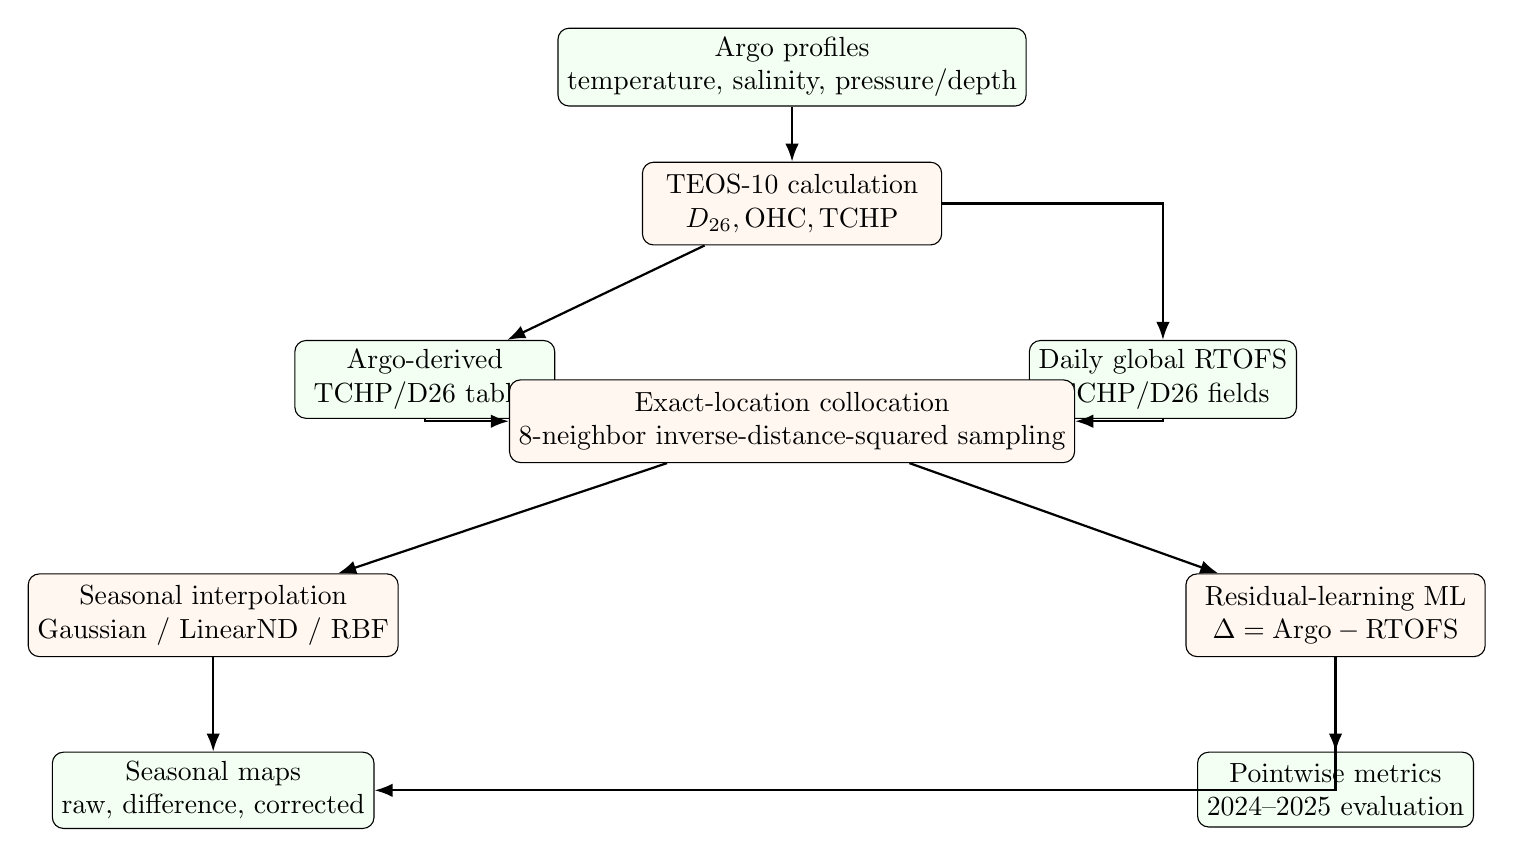
\begin{tikzpicture}[
  node distance=7mm and 8mm,
  box/.style={draw, rounded corners, align=center, minimum width=3.3cm, minimum height=0.95cm, fill=blue!4},
  data/.style={draw, rounded corners, align=center, minimum width=3.3cm, minimum height=0.95cm, fill=green!5},
  proc/.style={draw, rounded corners, align=center, minimum width=3.8cm, minimum height=1.05cm, fill=orange!6},
  arr/.style={-{Latex[length=2.3mm]}, thick}
]
\node[data] (argo) {Argo profiles\\temperature, salinity, pressure/depth};
\node[proc, below=of argo] (teos) {TEOS-10 calculation\\\(\Dtwentysix{}, \OHC, \TCHP\)};
\node[data, below left=12mm and 11mm of teos] (argoout) {Argo-derived\\TCHP/D26 tables};
\node[data, below right=12mm and 11mm of teos] (rtofs) {Daily global RTOFS\\TCHP/D26 fields};
\node[proc, below=17mm of teos] (colloc) {Exact-location collocation\\8-neighbor inverse-distance-squared sampling};
\node[proc, below left=14mm and 14mm of colloc] (interp) {Seasonal interpolation\\Gaussian / LinearND / RBF};
\node[proc, below right=14mm and 14mm of colloc] (ml) {Residual-learning ML\\\(\Delta = \text{Argo} - \text{RTOFS}\)};
\node[data, below=12mm of interp] (maps) {Seasonal maps\\raw, difference, corrected};
\node[data, below=12mm of ml] (metrics) {Pointwise metrics\\2024--2025 evaluation};

\draw[arr] (argo) -- (teos);
\draw[arr] (teos) -- (argoout);
\draw[arr] (argoout) |- (colloc);
\draw[arr] (rtofs) |- (colloc);
\draw[arr] (teos.east) -| (rtofs.north);
\draw[arr] (colloc) -- (interp);
\draw[arr] (colloc) -- (ml);
\draw[arr] (interp) -- (maps);
\draw[arr] (ml) -- (metrics);
\draw[arr] (ml) |- (maps);
\end{tikzpicture}
}
\caption{High-level HHP code schematic.}
\end{figure}

\chapter{TEOS-10 Calculation for \texorpdfstring{\Dtwentysix{}, \OHC{}, and \TCHP{}}{D26, OHC, and TCHP}}
\section{Core package dependencies}
The thermodynamic calculation is implemented in \code{OHC/teos\_ohc.py}. The main numerical dependencies are:
\begin{itemize}[leftmargin=1.3em]
  \item \code{gsw}: Gibbs SeaWater / TEOS-10 functions.
  \item \code{numpy}: profile cleaning, interpolation, masking, and vertical integration.
\end{itemize}

\section{Input conventions}
\begin{itemize}[leftmargin=1.3em]
  \item \code{vertical}: pressure in dbar for Argo-style profiles or depth in meters for RTOFS-style profiles.
  \item \code{temp\_c}: in-situ temperature profile in degrees Celsius.
  \item \code{salinity\_psu}: practical salinity profile.
  \item \code{lat, lon}: required by TEOS-10 conversions.
\end{itemize}

\section{Reference constants}
\begin{align}
T_{\mathrm{ref}} &= 26\celsius{} \\
\mathrm{J\,m^{-2}} \to \mathrm{kJ\,cm^{-2}} &= 10^{-7}
\end{align}
These are encoded in the code as:
\begin{lstlisting}[language=Python]
REF_TEMP_C = 26.0
J_PER_M2_TO_KJ_PER_CM2 = 1.0 / 1.0e7
\end{lstlisting}

\section{Mathematical definition}
\subsection{Depth of the 26-degree isotherm}
The code computes \Dtwentysix{} by scanning downward through the sorted profile. If the surface temperature is already below \(26\celsius{}\), the function returns no valid crossing.

For the first vertical pair \((z_1, T_1)\), \((z_2, T_2)\) such that \(T_1 > 26\celsius{}\) and \(T_2 \le 26\celsius{}\), the crossing depth is linearly interpolated:
\begin{equation}
\Dtwentysix{} = z_1 + \frac{T_1 - 26}{T_1 - T_2}(z_2 - z_1).
\end{equation}

\subsection{TEOS-10 heat-content integration}
Once the profile is truncated and interpolated to the exact \Dtwentysix{} crossing, the code converts practical salinity to absolute salinity and computes exact density and heat capacity:
\begin{align}
S_A &= \mathrm{SA\_from\_SP}(S_P, p, \lambda, \phi), \\
\rho &= \rho_t^{\mathrm{exact}}(S_A, T, p), \\
C_p &= C_p^{\mathrm{exact}}(S_A, T, p).
\end{align}

The volumetric heat excess above \(26\celsius{}\) is:
\begin{equation}
q(z) = \max\bigl(T(z) - 26, 0\bigr)\,\rho(z)\,C_p(z).
\end{equation}

The integrated ocean heat content above the isotherm is:
\begin{equation}
\OHC = \int_0^{\Dtwentysix{}} q(z)\,dz.
\end{equation}

The tropical cyclone heat potential is then:
\begin{equation}
\TCHP = \OHC \times 10^{-7} \quad [\mathrm{kJ\,cm^{-2}}].
\end{equation}

\section{Pseudocode for the main computation}
\begin{algorithm}[H]
\caption{TEOS-10 OHC/TCHP computation}
\begin{algorithmic}[1]
\Require vertical coordinate, temperature profile, practical salinity, latitude, longitude
\State Remove non-finite values and sort the profile by depth/pressure
\If{fewer than 2 valid levels}
    \State return no result
\EndIf
\If{input axis is pressure}
    \State convert pressure to depth using \code{gsw.z\_from\_p}
\Else
    \State convert depth to pressure using \code{gsw.p\_from\_z}
\EndIf
\State Find \Dtwentysix{} using downward crossing of \(26\celsius{}\)
\If{surface temperature is below \(26\celsius{}\) or no crossing exists}
    \State return \code{d26=None, tchp=None}
\EndIf
\State Interpolate temperature, salinity, and pressure to the exact \Dtwentysix{} depth
\State Convert practical salinity to absolute salinity with \code{gsw.SA\_from\_SP}
\State Compute exact density and heat capacity with \code{gsw.rho\_t\_exact} and \code{gsw.cp\_t\_exact}
\State Compute heat excess \(q(z)=\max(T-26,0)\rho C_p\)
\State Integrate \(q(z)\) from surface to \Dtwentysix{} using trapezoidal integration
\State Convert J/m\(^2\) to kJ/cm\(^2\)
\State return \Dtwentysix{}, \OHC{}, \TCHP{}
\end{algorithmic}
\end{algorithm}

\chapter{Why the Maps Concentrate in Warm-Water Regions}
Raw Argo coverage is global, but valid \Dtwentysix{} and \TCHP{} coverage is not. The physics-based filter is the \(26\celsius{}\) threshold.

\section{Observed evidence from the 2024 Argo subset}
\begin{table}[H]
\centering
\begin{tabular}{lrrrr}
\toprule
Subset & Raw Argo points & Raw points with $|\phi|>45^\circ$ & Valid D26/TCHP points & Valid high-latitude points \\
\midrule
Winter (JFM) & 38,693 & 10,804 & 11,133 & 0 \\
Summer (JAS) & 41,804 & 11,456 & 14,277 & 0 \\
\bottomrule
\end{tabular}
\caption{Raw Argo is global, but valid warm-water \Dtwentysix{}/\TCHP{} points vanish at high latitude.}
\end{table}

This means the equatorial and subtropical appearance of the final fields is a consequence of the target definition, not a consequence of missing Argo observations at higher latitude.

\chapter{Argo--RTOFS Collocation and Seasonal Interpolation}
\section{Exact-location sampling rationale}
The code intentionally avoids subtracting two independently gridded global surfaces directly. Instead, it first samples RTOFS at the exact Argo locations and dates. This keeps the statistical comparison tied to a shared point set.

\section{Native-grid neighbor sampling}
The collocation logic lives in two scripts:
\begin{itemize}[leftmargin=1.3em]
  \item \code{OHC/build\_rtofs\_at\_argo\_points\_surface\_diff\_2024.py}
  \item \code{OHC/build\_rtofs\_at\_argo\_points\_multiyear.py}
\end{itemize}
The key parameters are:
\begin{table}[H]
\centering
\small
\begin{tabular}{P{0.18\textwidth} P{0.15\textwidth} P{0.55\textwidth}}
\toprule
\textbf{Parameter} & \textbf{Value} & \textbf{Role} \\
\midrule
\code{K\_NEIGHBORS} & 8 & Number of nearest native RTOFS cells used for exact-location interpolation \\
Distance space & unit-sphere xyz & Enables \code{cKDTree} nearest-neighbor lookup on the globe \\
Weighting & $1/d^2$ & Inverse-distance-squared weighting for non-exact points \\
Exact threshold & $d \le 10^{-6}$ & If a point falls essentially on a grid cell, use that exact cell value \\
\bottomrule
\end{tabular}
\normalsize
\end{table}

\subsection{Distance conversion used in code}
Lat/lon are mapped to a unit sphere:
\begin{equation}
\mathbf{x}(\phi,\lambda) = 
\begin{bmatrix}
\cos\phi\cos\lambda \\
\cos\phi\sin\lambda \\
\sin\phi
\end{bmatrix}.
\end{equation}

For a unit-sphere chord distance \(c\), the great-circle distance in kilometers is:
\begin{equation}
d = \R \cdot 2\arcsin\left(\frac{c}{2}\right), \qquad \R = 6371\,\mathrm{km}.
\end{equation}

\section{Pseudocode for RTOFS-at-Argo collocation}
\begin{algorithm}[H]
\caption{Collocate RTOFS fields to exact Argo points}
\begin{algorithmic}[1]
\Require Argo table with date, latitude, longitude, target values
\Require Daily RTOFS TCHP/D26 fields on native model grid
\State Build a \code{cKDTree} from native RTOFS latitude/longitude converted to xyz coordinates
\For{each Argo point}
    \State Query the 8 nearest native RTOFS cells
    \State Convert chord distances to great-circle distances in km
    \If{an exact or nearly exact grid hit exists}
        \State assign the exact grid value
    \Else
        \State assign weighted mean using weights \(w_i = 1 / d_i^2\)
    \EndIf
\EndFor
\State Compute residuals: \(\Delta_{\TCHP} = \TCHP_{\mathrm{Argo}} - \TCHP_{\mathrm{RTOFS}}\), likewise for \Dtwentysix{}
\State Save collocated rows and derived fields
\end{algorithmic}
\end{algorithm}

\section{Surface interpolation methods tested}
The shared interpolation kernels live in \code{OHC/seasonal\_map\_common.py}.

\begin{table}[H]
\centering
\small
\begin{tabular}{P{0.20\textwidth} P{0.27\textwidth} P{0.37\textwidth}}
\toprule
Method & Implementation & Main parameters \\
\midrule
Gaussian & \code{gaussian\_interpolate()} & \(L=100\km,\;R=300\km\) \\
LinearND & \code{LinearNDInterpolator} & optional support mask \\
RBF Gaussian & \code{RBFInterpolator} & \(\epsilon=100\km,\;k=64,\;s=10^{-6}\) \\
\bottomrule
\end{tabular}
\normalsize
\end{table}

\section{The 100 km support mask}
The key map parameters used in the seasonal surface scripts are:
\begin{table}[H]
\centering
\begin{tabular}{lll}
\toprule
\textbf{Parameter} & \textbf{Value} & \textbf{Meaning} \\
\midrule
\code{GRID\_RES\_DEG} & 0.25 & Rendered global grid resolution \\
\code{MASK\_DISTANCE\_KM} & 100.0 & Support mask distance from nearest collocated observation \\
\code{length\_scale\_km} & 100.0 & Gaussian smoothing scale \\
\code{truncation\_radius\_km} & 300.0 & Gaussian neighborhood cutoff \\
\code{epsilon\_km} & 100.0 & Gaussian RBF kernel scale \\
\bottomrule
\end{tabular}
\end{table}

The mask logic is:
\begin{equation}
\text{grid node valid} \iff d_{\min}(\text{grid node},\text{observation set}) \le 100\km.
\end{equation}

The function \code{chord\_from\_km()} converts the 100 km radius to unit-sphere chord length:
\begin{equation}
c_{100} = 2\sin\left(\frac{100/6371}{2}\right).
\end{equation}

\subsection*{Important interpretation}
The 100 km mask is a \emph{support constraint}. It decides where the map is allowed to display values. It is not the same as the Gaussian length scale or RBF epsilon, which control the shape of the interpolation itself.

\section{Difference workflows that were explored}
\begin{enumerate}[leftmargin=1.4em]
  \item \textbf{Point-difference then interpolate:} compute \(\text{Argo} - \text{RTOFS}\) at collocated points first, then interpolate the difference field.
  \item \textbf{Interpolate surfaces then difference:} interpolate Argo and RTOFS-at-Argo-locations separately, then subtract the seasonal surfaces.
  \item \textbf{ML-corrected point predictions then interpolate:} predict corrected RTOFS values at collocated points, then render raw, corrected, and difference maps.
\end{enumerate}

\begin{figure}[H]
\centering
\resizebox{0.92\textwidth}{!}{
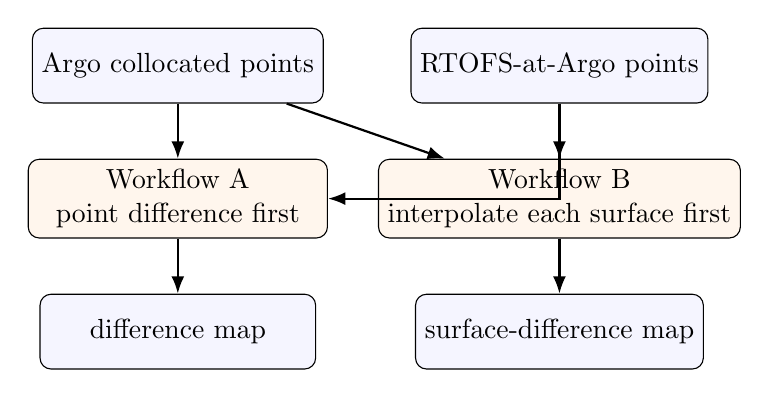
\begin{tikzpicture}[
  node distance=7mm and 11mm,
  box/.style={draw, rounded corners, align=center, minimum width=3.5cm, minimum height=0.95cm, fill=blue!4},
  proc/.style={draw, rounded corners, align=center, minimum width=3.8cm, minimum height=1.0cm, fill=orange!7},
  arr/.style={-{Latex[length=2.2mm]}, thick}
]
\node[box] (argo) {Argo collocated points};
\node[box, right=of argo] (rtofs) {RTOFS-at-Argo points};
\node[proc, below=of argo] (diff1) {Workflow A\\point difference first};
\node[proc, below=of rtofs] (surf) {Workflow B\\interpolate each surface first};
\node[box, below=of diff1] (map1) {difference map};
\node[box, below=of surf] (map2) {surface-difference map};
\draw[arr] (argo) -- (diff1);
\draw[arr] (rtofs) |- (diff1);
\draw[arr] (argo) -- (surf);
\draw[arr] (rtofs) -- (surf);
\draw[arr] (diff1) -- (map1);
\draw[arr] (surf) -- (map2);
\end{tikzpicture}
}
\caption{Two non-ML difference workflows explored before the ML correction stage.}
\end{figure}

\chapter{Machine-Learning Correction Pipeline}
\section{Training-table design}
The ML stage uses the multiyear collocation table from \path{OHC/build_rtofs_at_argo_points_multiyear.py}. It is a pointwise table, not an image dataset.

\begin{table}[H]
\centering
\begin{tabular}{lrr}
\toprule
Subset & Rows & Dates \\
\midrule
2024 collocated rows & 27,316 & 61 \\
2025 collocated rows & 14,031 & 29 \\
Combined 2024--2025 rows & 41,347 & 90 \\
Finite residual rows per target & 12,543 & 90-date universe \\
\bottomrule
\end{tabular}
\end{table}

\section{Residual-learning target}
For each collocated point, the ML model learns a correction term rather than a direct Argo prediction:
\begin{align}
\Delta_{\TCHP} &= \TCHP_{\mathrm{Argo}} - \TCHP_{\mathrm{RTOFS}}, \\
\Delta_{\Dtwentysix{}} &= \Dtwentysix{}_{\mathrm{Argo}} - \Dtwentysix{}_{\mathrm{RTOFS}}, \\
\widehat{y}_{\mathrm{corrected}} &= y_{\mathrm{raw\,RTOFS}} + \widehat{\Delta}.
\end{align}

\section{First benchmark family}
The first benchmark script is \code{OHC/benchmark\_rtofs\_argo\_tabular\_models.py}. It compares:
\begin{itemize}[leftmargin=1.3em]
  \item raw RTOFS baseline,
  \item mean residual baseline,
  \item ridge regression,
  \item random forest,
  \item gradient boosting,
  \item sklearn MLP,
  \item XGBoost,
  \item simple mean ensemble of nonlinear predictors.
\end{itemize}

\section{Leakage-aware split design}
The locked protocol, frozen in \code{OHC/output/ml\_benchmarks/locked\_protocol\_note.md}, uses:
\begin{itemize}[leftmargin=1.3em]
  \item split unit: \textbf{date},
  \item split type: \textbf{forward-chaining blocked validation},
  \item embargo: \textbf{1 date},
  \item folds: \textbf{3},
  \item random row splits: \textbf{forbidden}.
\end{itemize}

The reason is to reduce leakage from same-day spatial clustering and adjacent ocean states. This keeps the evaluation closer to a realistic forward-use scenario.

\section{Features used in the locked protocol}
\begin{table}[H]
\centering
\begin{tabular}{p{0.28\textwidth} p{0.62\textwidth}}
\toprule
\textbf{Feature block} & \textbf{Variables} \\
\midrule
Time encoding & \code{year}, \code{month\_int}, \code{month\_sin}, \code{month\_cos}, \code{doy\_sin}, \code{doy\_cos} \\
Location & \code{lat}, \code{lon}, \code{abs\_lat} \\
Sampling geometry & \code{nearest\_rtofs\_grid\_distance\_km} \\
Season indicator & \code{is\_winter\_jfm}, \code{is\_summer\_jas}, \code{is\_other} \\
Model-state context & \code{model\_interp\_tchp\_kj\_per\_cm2}, \code{model\_interp\_d26\_m} \\
\bottomrule
\end{tabular}
\end{table}

\section{Pseudocode for the year-holdout ML path}
\begin{algorithm}[H]
\caption{2024-train / 2025-test XGBoost correction}
\begin{algorithmic}[1]
\Require multiyear collocation table with Argo observations, raw RTOFS-at-Argo values, and residual targets
\State Keep only rows with finite Argo target, finite raw RTOFS target, and finite residual target
\State Build engineered features from date, season, location, and raw model state
\State Split rows by year: train on 2024, test on 2025
\State Fit preprocessing pipeline (median imputation; no scaling for tree models)
\State Train XGBoost regressor on the residual target \(\Delta\)
\State Predict residuals on 2025 rows
\State Form corrected prediction: \(\widehat{y}_{\mathrm{corr}} = y_{\mathrm{raw}} + \widehat{\Delta}\)
\State Compute MAE, RMSE, bias, and correlation against Argo at 2025 collocated points
\State Group results by season and region
\end{algorithmic}
\end{algorithm}

\section{Strongest current model and exact hyperparameters}
\subsection{Locked benchmark model}
The strongest practical single-model baseline is XGBoost with:
\begin{lstlisting}[language=Python]
XGBRegressor(
    random_state=0,
    n_estimators=400,
    max_depth=5,
    learning_rate=0.05,
    subsample=0.8,
    colsample_bytree=0.8,
    reg_lambda=1.0,
    objective="reg:squarederror",
    n_jobs=8,
)
\end{lstlisting}

\subsection{Best year-holdout sweep models}
The year-holdout sweep uses the same 2024-train / 2025-test setup plus an inner blocked time-validation step. The best models found were:
\begin{itemize}[leftmargin=1.3em]
  \item \textbf{TCHP:} enriched feature set, 3 inner folds, with \(n_\mathrm{est}=300\), depth \(=4\), rate \(=0.03\), and subsample / colsample \(=0.8\).
  \item \textbf{D26:} base feature set, same XGBoost hyperparameters.
\end{itemize}

\section{Feature-enrichment logic in the sweep}
The sweep script adds the following beyond the base features:
\begin{itemize}[leftmargin=1.3em]
  \item coarse region indicators: Atlantic, Indian, Pacific, northern high latitude, southern high latitude,
  \item warm-water availability flags,
  \item interaction terms such as \code{model\_tchp\_x\_abs\_lat} and \code{model\_d26\_x\_abs\_lat}.
\end{itemize}

\section{Current benchmark performance}
\subsection{Locked forward-chaining benchmark}
\begin{table}[H]
\centering
\begin{tabular}{llrrrr}
\toprule
Target & Model & MAE & RMSE & Bias & Corr. \\
\midrule
D26 & Raw RTOFS & 14.61 & 19.86 & -7.28 & 0.888 \\
D26 & Locked XGBoost & 10.94 & 14.71 & -0.54 & 0.928 \\
TCHP & Raw RTOFS & 16.26 & 22.64 & -8.97 & 0.915 \\
TCHP & Locked XGBoost & 11.86 & 16.73 & 0.39 & 0.944 \\
\bottomrule
\end{tabular}
\caption{Official locked out-of-fold summary over 2024--2025 blocked folds.}
\end{table}

\subsection{Year-holdout train-2024 / test-2025 summary}
\begin{table}[H]
\centering
\begin{tabular}{lrrr}
\toprule
Target & Raw RTOFS MAE & Best corrected MAE & Improvement \\
\midrule
TCHP & 16.17 & 11.71 & 4.46 \\
D26 & 14.82 & 11.55 & 3.28 \\
\bottomrule
\end{tabular}
\caption{Best 2024-train / 2025-test correction performance at collocated points.}
\end{table}

\begin{figure}[H]
\centering
\resizebox{0.88\textwidth}{!}{
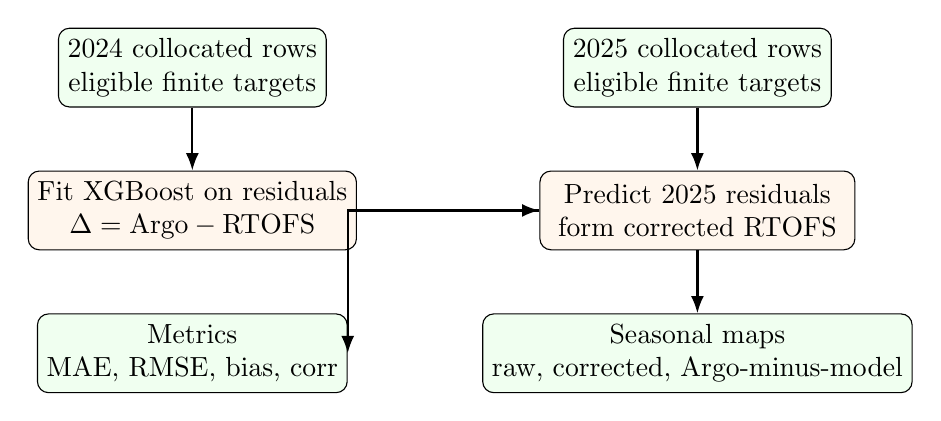
\begin{tikzpicture}[
  node distance=8mm and 9mm,
  box/.style={draw, rounded corners, align=center, minimum width=3.4cm, minimum height=1.0cm, fill=green!6},
  proc/.style={draw, rounded corners, align=center, minimum width=4cm, minimum height=1.0cm, fill=orange!7},
  arr/.style={-{Latex[length=2.2mm]}, thick}
]
\node[box] (train) {2024 collocated rows\\eligible finite targets};
\node[box, right=30mm of train] (test) {2025 collocated rows\\eligible finite targets};
\node[proc, below=of train] (fit) {Fit XGBoost on residuals\\\(\Delta=\text{Argo}-\text{RTOFS}\)};
\node[proc, below=of test] (pred) {Predict 2025 residuals\\form corrected RTOFS};
\node[box, below=of fit] (metrics) {Metrics\\MAE, RMSE, bias, corr};
\node[box, below=of pred] (maps) {Seasonal maps\\raw, corrected, Argo-minus-model};
\draw[arr] (train) -- (fit);
\draw[arr] (test) -- (pred);
\draw[arr] (fit.east) -- ++(1.4,0) |- (pred.west);
\draw[arr] (pred) -- (maps);
\draw[arr] (pred.west) -| (metrics.east);
\end{tikzpicture}
}
\caption{Year-holdout ML schematic used for the current strongest correction workflow.}
\end{figure}

\chapter{Key Interpretive Points}
\begin{enumerate}[leftmargin=1.4em]
  \item The warm-water appearance of the final \Dtwentysix{}/\TCHP{} maps is caused by the \(26\celsius{}\) threshold and not by a lack of global Argo coverage.
  \item The 100 km mask is a support mask that suppresses display where collocated observations are too far away; it is not the same as the smoothing kernel scale.
  \item The current machine-learning pipeline is a point-collocated residual-learning system, not yet a gridded deep-learning system.
  \item The current strongest deployable path is the year-holdout XGBoost correction trained on 2024 and tested on 2025.
\end{enumerate}

\chapter*{Appendix: Main artifact paths}
\addcontentsline{toc}{chapter}{Appendix: Main artifact paths}
\small
\begin{itemize}[leftmargin=1.4em]
  \item Raw Argo distribution summary:\\ \path{OHC/output/argo_raw_2024_distribution/summary_2024_raw_distribution.json}
  \item 2024 surface-difference summary:\\ \path{OHC/output/rtofs_at_argo_points_2024_surface_diff/data/summary_2024_winter_summer.json}
  \item Multiyear collocation summary:\\ \path{OHC/output/ml_collocation/data/summary_collocation_2024_2025.json}
  \item Locked evaluation protocol:\\ \path{OHC/output/ml_benchmarks/locked_protocol_note.md}
  \item Locked XGBoost OOF summary:\\ \path{OHC/output/ml_benchmarks/locked_xgb_oof_summary.csv}
  \item Year-holdout sweep best summary:\\ \path{OHC/output/ml_benchmarks/year_holdout_xgb_sweep_best_summary.csv}
\end{itemize}
\normalsize

\end{document}
